% The main thesis file
% Don't put any content in here. 
% Don't even include content files by using \input or \inlcude. 
% Put your content to text.tex or include it there using \input.
% Uses:
%       SETTINGS.TEX        contains the settings for this document
%       COMMANDS.TEX        contains commands which can be used while writing
%       INFO.TEX            contains the author, title and so on for the cover
%       COVER.TEX           formats the front cover of the document
%       ABSTRACT.TEX        contains the abstract to be included (if needed)
%       TEXT.TEX            contains the actual content of the document
%       BIB.BIB             contains the BibTeX entries for the document

%% Draft document mode
%% Final document
\documentclass[11pt,a4paper,bibtotoc,idxtotoc,headsepline,footsepline,footexclude,BCOR12mm,DIV13]{scrbook}

%\documentclass[11pt,a4paper,bibtotoc,idxtotoc,headsepline,footsepline,footexclude,BCOR20mm,DIV10]{scrbook}

% KOMA-Optionen:
%  bibtotoc: include bibliography in table of contents
%  idxtotoc: include index in table of contents
%  headsepline: use horizontalline under heading
%  BCOR: binding correcion (Bindungskorrektur) (e.g.: BCOR5mm)
%  DIV: Number of sheet sections (used for layout) (e.g.: DIV12) 


% include title and author information for the cover
% Set here the title, authors and other stuff to be used for the cover
% This file is used by main.tex

% set title, authors and stuff for the cover
\def\doctype{Master's Thesis in Informatics}
\def\title{Utilizing Crowd Intelligence for Online Detection of Emotional Distress}
\def\titleGer{Die Verwendung von Crowd Intelligence zur unmittelbaren Erkennung von emotionalem Stress}
\def\author{Siddhant Goel}
\def\date{March 15, 2013}

% text to appear in the footer
\def\footertext{}


% include settings
% Included by main.tex
% Defines the settings for the thesis

\renewcommand{\sectfont}{\normalfont \bfseries}        % Schriftart der Kopfzeile

% manipulate footer
\usepackage{scrpage2}
\pagestyle{scrheadings}
\ifoot[\footertext]{\footertext} % \footertext set in INFO.TEX
%\setkomafont{pagehead}{\normalfont\rmfamily}
\setkomafont{pagenumber}{\normalfont\rmfamily}

%% allow sophisticated control structures
\usepackage{ifthen}

% use Palatino as default font
\usepackage{palatino}

% enable special PostScript fonts
\usepackage{pifont}

% make thumbnails
\usepackage{thumbpdf}

%to use the subfigures
\usepackage{subfigure}

\usepackage{colortbl}

%% show program code\ldots
%\usepackage{verbatim}
%\usepackage{program}

%% enable TUM symbols on title page
\usepackage{styles/tumlogo}

\usepackage{multirow}

%% use colors
\usepackage{color}

%% make fancy math
\usepackage{amsmath}
\usepackage{amsfonts}
\usepackage{amssymb}
\usepackage{textcomp}
\usepackage{yhmath} % f�r die adots 
%% mark text as preliminary
%\usepackage[draft,german,scrtime]{prelim2e}

%% create an index
\usepackage{makeidx}

% for the program environment
\usepackage{float}

%% load german babel package for german abstract
%\usepackage[german,american]{babel}
\usepackage[german,english]{babel}
\selectlanguage{english}

% use german characters as well
\usepackage[latin1]{inputenc}       % allow Latin1 characters

% use initals dropped caps - doesn't work with PDF
\usepackage{lettrine}

\usepackage{styles/shortoverview}
%----------------------------------------------------
%      Graphics and Hyperlinks
%----------------------------------------------------

%% check for pdfTeX
\ifx\pdftexversion\undefined
%% use PostScript graphics
\usepackage[dvips]{graphicx}
\DeclareGraphicsExtensions{.eps,.epsi}
\graphicspath{{figures/}{figures/review}} 
%% allow rotations
\usepackage{rotating}
%% mark pages as draft copies
%\usepackage[english,all,light]{draftcopy}
%% use hypertex version of hyperref
\usepackage[hypertex,hyperindex=false,colorlinks=false]{hyperref}
\else %% reduce output size \pdfcompresslevel=9
%% declare pdfinfo
%\pdfinfo { 
%  /Title (my title) 
%  /Creator (pdfLaTeX) 
%  /Author (my name) 
%  /Subject (my subject	) 
%  /Keywords (my keywords)
%}
%% use pdf or jpg graphics
\usepackage[pdftex]{graphicx}
\DeclareGraphicsExtensions{.jpg,.JPG,.png,.pdf,.eps}
\graphicspath{{figures/}} 
 
%% Load float package, for enabling floating extensions
\usepackage{float}
 
%% allow rotations
\usepackage{rotating}
%% use pdftex version of hyperref
\usepackage[pdftex,colorlinks=false,linkcolor=red,citecolor=red,%
anchorcolor=red,urlcolor=red,bookmarks=true,%
bookmarksopen=true,bookmarksopenlevel=0,plainpages=false%
bookmarksnumbered=true,hyperindex=false,pdfstartview=%
]{hyperref}
%
%\usepackage[pdftex,colorlinks=false,linkcolor=red,citecolor=red,%
% anchorcolor=red,urlcolor=red,bookmarks=true,%
% bookmarksopen=true,bookmarksopenlevel=0,plainpages=false%
% bookmarksnumbered=true,hyperindex=false,pdfstartview=%
% ]{hyperref}
\fi

%% Fancy chapters
\usepackage[Lenny]{fncychap}
% \usepackage[Glenn]{fncychap}
% \usepackage[Bjarne]{fncychap}

%\usepackage[avantgarde]{quotchap}

% set the bibliography style
%\bibliographystyle{styles/bauermaNum}
%\bibliographystyle{alpha}
\bibliographystyle{plain}


% include commands
% Commands to be used within the TUM report document
% Included by main.tex
% Please include your own cool commands here. 
% Be only sure to comment it sufficiently so others can use it.

%-------------------------------------------------------------
%                      Own Commands
%-------------------------------------------------------------

%-------------------------------------------------------------
% math stuff -------------------------------------------------

% nice R, N, C
\newcommand{\nat}{\mathbb{N}}
\newcommand{\real}{\mathbb{R}}
\newcommand{\compl}{\mathbb{C}}

% norm
\newcommand{\norm}[1]{\left\| #1 \right\|}

% un demi
\newcommand{\half}{\frac{1}{2}}

% parantheses
\newcommand{\parenth}[1]{ \left( #1 \right) }
\newcommand{\bracket}[1]{ \left[ #1 \right] }
\newcommand{\accolade}[1]{ \left\{ #1 \right\} }
%\newcommand{\angle}[1]{ \left\langle  #1 \right\rangle }

% partial derivative: %#1 function, #2 which variable
% simple / single line version
\newcommand{\pardevS}[2]{ \delta_{#1} f(#2) }
% fraction version
\newcommand{\pardevF}[2]{ \frac{\partial #1}{\partial #2} }

% render vectors: 3 and 4 dimensional
\newcommand{\veciii}[3]{\left[ \begin{array}[h]{c} #1 \\ #2 \\ #3	\end{array} \right]}
\newcommand{\veciv}[4]{\left[ \begin{array}[h]{c} #1 \\ #2 \\ #3 \\ #4	\end{array} \right]}

% render matrices: 3  dimensional (arguments in row first order)
\newcommand{\matiii}[9]{\left[ \begin{array}[h]{ccc} #1 & #2 & #3 \\ #4 & #5 & #6 \\ #7 & #8 & #9	\end{array} \right]}

%-------------------------------------------------------------
% some abbreviations ------------------------------------------
\newcommand{\Reg}{$^{\textregistered}$}
\newcommand{\reg}{$^{\textregistered}$ }
\newcommand{\Tm}{\texttrademark}
\newcommand{\tm}{\texttrademark~}
\newcommand {\bsl} {$\backslash$}

%-------------------------------------------------------------
%-------------------------------------------------------------

%-------------------------------------------------------------
% formatting --------------------------------------------------

% Theorem & Co environments and counters
\newtheorem{theorem}{Theorem}[chapter]
\newtheorem{lemma}[theorem]{Lemma}
\newtheorem{corollary}[theorem]{Corollary}
\newtheorem{remark}[theorem]{Remark}
\newtheorem{definition}[theorem]{Definition}
\newtheorem{equat}[theorem]{Equation}
\newtheorem{example}[theorem]{Example}
\newtheorem{algorithm}[theorem]{Algorithm}

% inserting figures
\newcommand{\insertfigure}[4]{ % Filename, Caption, Label, Width percent of textwidth
\begin{figure}[htbp]
    \begin{center}
        \includegraphics[width=#4\textwidth]{#1}
    \end{center}
    \vspace{-0.4cm}
    \caption{#2}
    \label{#3}
\end{figure}
}

% referecing figures

\newcommand{\refFigure}[1]{ %label
figure \ref{#1}
}
\newcommand{\refChapter}[1]{ %label
chapter \ref{#1}
}

\newcommand{\refSection}[1]{ %label
section \ref{#1}
}

\newcommand{\refParagraph}[1]{ %label
paragraph \ref{#1}
}

\newcommand{\refEquation}[1]{ %label
equation \ref{#1}
}

\newcommand{\refTable}[1]{ %label
table \ref{#1}
}

\newcommand{\rigidTransform}[2]
{
${}^{#2}\!\mathbf{H}_{#1}$
}

%code, in typewriter
\newcommand{\code}[1]
{\texttt{#1}}

% comment that appears on the border - very practical !!!
\newcommand{\comment}[1]{\marginpar{\raggedright \noindent \footnotesize {\sl #1} }}

% page clearing
\newcommand{\clearemptydoublepage}{%
\ifthenelse{\boolean{@twoside}}{\newpage{\pagestyle{empty}\cleardoublepage}}%
{\clearpage}}

%-------------------------------------------------------------
%-------------------------------------------------------------

\newcommand{\etAl}{\emph{et al.}\mbox{ }}


%\makeindex
%% inter line spacing
%\linespread{1.0}

\makeglossary

\begin{document}
    \frontmatter
    % The front cover for the TUM report document.
% Included by main.tex

%--------------------------------------------------
% The Front Cover
%--------------------------------------------------

% correct BCOR - undo at the end !!!
\def\bcorcor{0.15cm}
\addtolength{\hoffset}{\bcorcor}

\thispagestyle{empty}

\vspace{4cm}
\begin{center}
    \oTUM{4cm}\\
    \vspace{5mm}
    \huge FAKULT{\"A}T F{\"U}R INFORMATIK\\ 
    \vspace{0.5cm}
    \large DER TECHNISCHEN UNIVERSIT{\"A}T M{\"U}NCHEN\\
    \vspace{1mm}
\end{center}

\vspace{15mm}
\begin{center}
    {\Large \doctype}
    
    \vspace{20mm}
    
    {\huge\bf \title}\\%[3ex]
    
    \vspace{15mm}
    
    {\LARGE  \author}
    
    \vspace{10mm}
    
    \begin{figure}[h!]
        \centering
        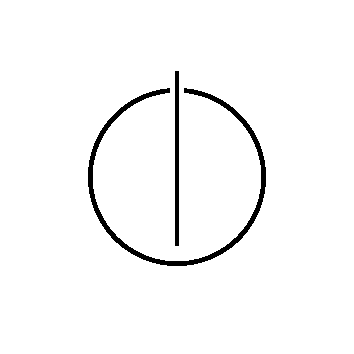
\includegraphics[width=4cm]{styles/informat.png}
    \end{figure}
\end{center}

    %	\clearemptydoublepage
    %	
    %	% The titlepage for the thesis
% Included by main.tex

%--------------------------------------------------
% The title page
%--------------------------------------------------

% correct BCOR - undo at the end !!!
\def\bcorcor{0.15cm}
\addtolength{\hoffset}{\bcorcor}

\thispagestyle{empty}

\vspace{10mm}
\begin{center}
    \oTUM{4cm}
    \vspace{5mm}     
    \huge FAKULT{\"A}T F{\"U}R INFORMATIK\\ 
    \vspace{0.5cm}
    \large DER TECHNISCHEN UNIVERSIT{\"A}T M{\"U}NCHEN\\
\end{center}

\vspace{10mm}
\begin{center}
    {\Large \doctype}
    
    \vspace{10mm}
    
    {\LARGE \title}\\
    
    \vspace{10mm}
    
    {\LARGE  \titleGer}\\
    
    \vspace{10mm}
    
    %\hfill
    \begin{tabular}{ll}
        \Large Author:     & \Large \author \\[2mm]
        \Large Supervisor:    & \Large Prof. Dr. Claudia Eckert \\[2mm]
        \Large Advisor: & \Large Han Xiao, M.Sc. \\[2mm]
        \Large Date:       & \Large March 15, 2013
    \end{tabular}
    
    \vspace{5mm}
    
    \begin{figure}[h!]
        \centering
        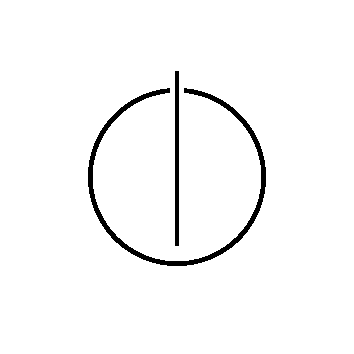
\includegraphics[width=4cm]{styles/informat.png}
    \end{figure}

\end{center}

% undo BCOR correction
\addtolength{\hoffset}{\bcorcor}

    %	\input{components/cover_maschmeyer}
    \clearemptydoublepage
    % The titlepage for the thesis
% Included by main.tex

%--------------------------------------------------
% The title page
%--------------------------------------------------

% correct BCOR - undo at the end !!!
\def\bcorcor{0.15cm}
\addtolength{\hoffset}{\bcorcor}

\thispagestyle{empty}

\vspace{10mm}
\begin{center}
    \oTUM{4cm}
    \vspace{5mm}     
    \huge FAKULT{\"A}T F{\"U}R INFORMATIK\\ 
    \vspace{0.5cm}
    \large DER TECHNISCHEN UNIVERSIT{\"A}T M{\"U}NCHEN\\
\end{center}

\vspace{10mm}
\begin{center}
    {\Large \doctype}
    
    \vspace{10mm}
    
    {\LARGE \title}\\
    
    \vspace{10mm}
    
    {\LARGE  \titleGer}\\
    
    \vspace{10mm}
    
    %\hfill
    \begin{tabular}{ll}
        \Large Author:     & \Large \author \\[2mm]
        \Large Supervisor:    & \Large Prof. Dr. Claudia Eckert \\[2mm]
        \Large Advisor: & \Large Han Xiao, M.Sc. \\[2mm]
        \Large Date:       & \Large March 15, 2013
    \end{tabular}
    
    \vspace{5mm}
    
    \begin{figure}[h!]
        \centering
        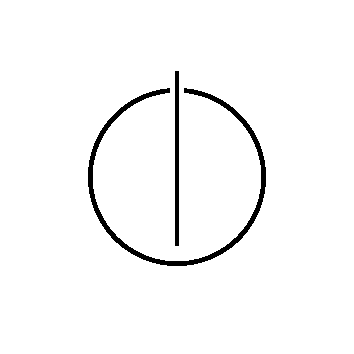
\includegraphics[width=4cm]{styles/informat.png}
    \end{figure}

\end{center}

% undo BCOR correction
\addtolength{\hoffset}{\bcorcor}

    \clearemptydoublepage

\thispagestyle{empty}
\selectlanguage{german}
\vspace*{0.8\textheight}
\noindent
Ich versichere, dass ich diese Diplomarbeit selbst{\"a}ndig verfasst und nur die angegebenen \\Quellen und Hilfsmittel verwendet habe.

I assure the single handed composition of this master's thesis only supported by declared resources.

\vspace{15mm}
\noindent
M{\"u}nchen, den \date \hspace{5cm} \author
\selectlanguage{english}
\newpage

    \clearemptydoublepage
\phantomsection
\addcontentsline{toc}{chapter}{Acknowledgements}	

%\chapter*{Acknowledgements}

\vspace*{2cm}

\begin{center}
{\Large \bf Acknowledgments}
\end{center}

\vspace{1cm}

I would like to thank my advisor Han Xiao, for being an incredible mentor. His guidance, critique, motivation, and above all, time, has led this project to a fruitful completion within the stipulated period of time. I would also like to thank Huang Xiao, who took out time from his schedule to help me set up the demo for this project. I also owe my deepest gratitude to the people behind the open source libraries including numpy, scipy, scikit-learn, libsvm, and django that made this project possible. Lastly, I would like to thank my family and friends, for providing continuous and unconditional support in all the endeavours that I undertook in the past, including this work.

    % Abstract for the TUM report document
% Included by main.tex

\clearemptydoublepage
\phantomsection
\addcontentsline{toc}{chapter}{Abstract}

\vspace*{2cm}
\begin{center}
{\Large \bf Abstract}
\end{center}
\vspace{1cm}

According to the World Health Organization, nearly one million people die from suicide every year. This means one death almost every 40 seconds. The maximum number of people committing suicide are between 15 and 29 years old, which comprises the young section of the society. The recent success of social networking websites like Twitter, Facebook, Reddit, and Wordpress has shown that more and more young people these days tend to express their inner feelings on the web, irrespective of whether those feelings are positive or negative. In order to bridge the disconnect between these two pieces of information, we present a surveillance and monitoring system of suicide.\\

The system blends supervised machine learning techniques and semi-online learning to make predictions about a general level of distress (in \%) amongst people posting on Twitter, and about particular instances of tweets which may lead one to believe that the author posting that content is depressed and may need further attention. The system also taps into crowd intelligence to learn about which pieces of text are depressed and which are not. In addition, we also present an evaluation of support vector machines and ensemble learning methods in the domains of text classification and sentiment analysis. The goal of the final system is to provide timely intervention and to promote better public health.

    \tableofcontents
    \clearemptydoublepage

\phantomsection
\addcontentsline{toc}{chapter}{Outline of the Thesis}

\begin{center}
    \huge{Outline of the Thesis}
\end{center}

%--------------------------------------------------------------------
\section*{Part I: Introduction}

\noindent {\scshape Chapter 1: Introduction}  \vspace{1mm}
\noindent  This chapter presents an overview of the thesis, and defines the problem which it aims to solve. \\

\noindent {\scshape Chapter 2: Related Work}  \vspace{1mm}
\noindent Related Work \\

%--------------------------------------------------------------------
\section*{Part II: Theoretical Background}

\noindent {\scshape Chapter 1: Classification Methods}  \vspace{1mm} \\

\noindent {\scshape Chapter 2: Text Representation}  \vspace{1mm} \\

\noindent {\scshape Chapter 3: Ensemble Learning}  \vspace{1mm} \\

%--------------------------------------------------------------------
\section*{Part III: Experiments}
\noindent {\scshape Chapter 1: Experiments}  \vspace{1mm} \\

\noindent {\scshape Chapter 2: Results}  \vspace{1mm} \\

%--------------------------------------------------------------------
\section*{Part IV: Conclusion}
\noindent {\scshape Chapter 1: Conclusion}  \vspace{1mm} \\

    \mainmatter
    % ---------------------------------------------------------------------------
    %
    %Introduction and Background Theory
    %
    % ---------------------------------------------------------------------------
    \part[Introduction and Theory]{Introduction and Theory}
    \label{part:introAndBackgroundTheory}
    \chapter{Introduction}
\label{chapter:Introduction}

Here starts the thesis with an introduction. Please use nice latex and bibtex entries \cite{latex}. Do not spend time on formating your thesis, but on its content.
 
\section{Latex Introduction}
There is no need for a latex introduction since there is plenty of literature out there.

    %
    %% ---------------------------------------------------------------------------
    %%
    %% Fully Automated Calibration for Ultrasound
    %%
    %%% ---------------------------------------------------------------------------
    \part[The 2nd Part]{The Second Part}
    \label{part:secondP}
    % ---------------------------------------------------------------------------
    %
    % Appendix
    %
    % ---------------------------------------------------------------------------
    \part*{Appendix}
    \addcontentsline{toc}{part}{Appendix}
    \appendix %---------------------------------------
    \chapter{Detailed Descriptions}
%\section{Detailed Validation Results}
\label{chapter:DetailedDescriptions}
Here come the details that are not supposed to be in the regular text.

    \clearemptydoublepage
    \bibliography{bibliography/literature}
\end{document}
